\documentclass{article}
\usepackage{graphicx} % Required for inserting images
\usepackage{amsmath}
\usepackage{amsfonts}
\DeclareMathOperator*{\argmax}{arg\,max}
\DeclareMathOperator*{\argmin}{arg\,min}

\usepackage{tikz}

\newcommand*{\xMin}{0}%
\newcommand*{\xMax}{4}%
\newcommand*{\yMin}{0}%
\newcommand*{\yMax}{4}%

\usetikzlibrary{positioning}% for specifications like "left=of ..."
\usetikzlibrary{automata}% automata related stuff
\usetikzlibrary{calc}% for calculating coordinates, like ($...$)
\usetikzlibrary{arrows.meta}% arrow head Stealth[round]

% define settings common to several automata
\tikzset{FAstyle/.style={
    shorten >=1pt,% leave a thin space between arrow head and target node
    node distance=3cm,% grid size
    on grid,% arrange nodes on a grid
    auto,% automatic placements of labels
    every state/.style={% define appearance of nodes
      draw=blue!50,
      very thick,
      top color=white,
      bottom color=blue!20,
      minimum size=0pt
    },
    >=Stealth[round],
    thick,
    draw=black!50
  }
}

\title{DS 598 HW1}
\author{Write your name here}

\begin{document}

\maketitle

\paragraph{Instructions:} Please submit a Jupyter notebook containing the code and the requested plots to the blackboard submission portal. You can make use of any open-sourced code as you wish, but you will be responsible for the correctness of the code you submit.

\begin{figure}[!h]
\centering
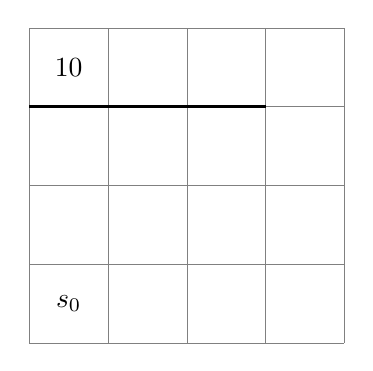
\begin{tikzpicture}
    \foreach \i in {\xMin,...,\xMax} {
        \draw [very thin,gray] (\i,\yMin) -- (\i,\yMax);
    }
    \foreach \i in {\yMin,...,\yMax} {
        \draw [very thin,gray] (\xMin,\i) -- (\xMax,\i);
    }
    \draw [very thick,black] (0,3) -- (3,3);
    
    \node at (0.5,0.5) {$s_0$};
    \node at (0.5,+3.5) {10};
\end{tikzpicture}
\caption{MDP.}
\end{figure}

\paragraph{Problem 1.} Implement the MDP using the gym Env class. The game resets once the agent finds the treasure ($r=10$). $\gamma = 0.9$. Each state has $4$ actions which moves left, right, up and down, respectively. If the agent moves against a wall, it will remain in the current state.


\paragraph{Problem 2.} Implement the DQN algorithm (with experience replay and target network) with $\epsilon$-greedy exploration, i.e. the agent use the action $a_t = \argmax_a Q_t(s_t)$ with probability $1-\epsilon$ and $a_t = \text{Unif}(A)$ with probability $\epsilon$. You are free to tune $\epsilon$ as well as other hyper-parameters in DQN as you wish. Use a two-layer MLP for the Q-network. 
\begin{itemize}
    \item Plot the learning curve averaging over 10 runs. The learning curve measures the performance of the policy $J(\pi_t)$ as a function of episode index $t$.
    \item Implement double DQN, and plot its learning curve in the same graph as above.
\end{itemize}


\paragraph{Problem 3.} Implement the vanilla REINFORCE algorithm using a two-layer MLP network with softmax output layer. You can tune the mini-batch size and learning rate as you wish.
\begin{itemize}
    \item Plot the learning curve averaging over 10 runs.
    \item Plot the learning curve using the $V^*$ function as a baseline for variance reduction.
    \item Plot the empirical variance of policy gradient with and without baseline. Given a set of trajectories $\tau_{1:n}$ from a policy $\pi_t$, the empirical variance is 
    \begin{align*}
        v_t= \frac{1}{n} \sum_{i=1}^n ||g_{t;i}-g_t||_2^2
    \end{align*}
    where 
    \begin{align*}
    g_{t;i}&=\sum_{h=0}^\infty \nabla_\theta\log\pi(a_{i;h}|s_{i;h}) (R(s_{i;h},a_{i;h})- \text{baseline}(s_{i;h}))\\
    g_t &= \frac{1}{n} \sum_{i=1}^n g_{t;i}
    \end{align*}
\end{itemize}

\end{document}

